% Template for ICIP-2019 paper; to be used with:
%          spconf.sty  - ICASSP/ICIP LaTeX style file, and
%          IEEEbib.bst - IEEE bibliography style file.
% --------------------------------------------------------------------------
\documentclass{article}
\usepackage{physics}
\usepackage{spconf,amsmath, amssymb, graphicx, url}
\usepackage{enumitem, booktabs, multirow}
\usepackage[table,xcdraw]{xcolor}
\usepackage{arydshln}
\usepackage{cite}

\usepackage{algorithm} 
\usepackage{algpseudocode} 

% \usepackage{caption}
% \captionsetup[table]{justification=centerlast,
%                      labelsep=newline,
%                      font=sf,
%                      textfont=footnotesize}
% \captionsetup[figure]{justification=centerlast,
%                      font=sf,
%                      textfont=footnotesize}

\DeclareMathOperator*{\argmax}{arg\,max}
\renewcommand\thetable{\Roman{table}} %Make the table's captions Roman numerals
% \setlength{\parskip}{0.1em}

%\parskip 0.2in %Separation between paragraphs
% Example definitions.
% --------------------
\def\x{{\mathbf x}}
\def\L{{\cal L}}
\def\-{\raisebox{.75pt}{-}}
% \renewcommand\thesubsection{\alph{subsection}} %Change subsection from using arabic to alphabetical numbering
% Title.
% ------
\title{System Design SYDE-675 Final Project: Multi-class AdaBoost for the classification of the Human Activity Recognition Dataset}
%
% Single address.
% ---------------
\name{Gomez Gonzalez, Juan M.}
% For example:
% ------------
\address{University of Waterloo\\
	Department of Electrical and Computer Engineering}

\begin{document}
%\ninept
%
\maketitle

\begin{abstract}
\ninept
\textbf{
This document is the solution for the Final Project of the System Design course SYDE-675, which was taught during the Winter of 2020 at University of Waterloo. It is based on the solutions found using Python, which can be found accompanying this document.
} 
\end{abstract}
%
\begin{keywords}
\ninept
Adaboost, AdaBoost SAMME, Support Vector Machines (SVMs), Decision Trees, Random Forests, K Nearest Neighbors (KNN).
\end{keywords} 

\section{Question 3: Paper Review}
\label{sec:Q3}
\subsection{Boosting}
The boosting meta-algorithm is considered to be one of the most powerful techniques for solving classification problems that has been developed in the last 20 years \cite{statisticalLearning}. Its premise is that by combining multiple weak learners, i.e. classifiers that have an accuracy larger than a coin toss ($50\%$), a more accurate learner can be created, at the same time that it reduces the possibility of overfitting on the training data \cite{Schapire_boosting}. Even though this seemed like a promising technique, it only began gaining traction with the development of the AdaBoost algorithm \cite{statisticalLearning}. It also differs from the bagging approach in the random forest classifier in that the latter focuses on using a random sampling with no changes in weights for each classifier, which means that all of the learners of the system have the same voting power \cite{Breinan_random_forests}.

\subsection{AdaBoost}
The AdaBoost differs from traditional boosting techniques in that the former adjusts on the fly to the errors that the weak learners have, giving the misclassifications a larger weight and thus making them more important \cite{Schapire_explaining_adaboost, Freund_adaboost}. This results in a simple yet powerful learner useful in multiple scenarios \cite{Schapire_explaining_adaboost}. However, the main disadvantage of this algorithm is that in its original form it is only capable of classifying binary classification problems. There are two possible solutions or approaches that can be done to resolve this issue: applying binary reduction or using a multi-class algorithm/modification \cite{Saberian_binarization_problems, Zhai_multiclass_boosting}. The former involves strategies like using multiple binary classifiers in a one versus one or one versus all approach, while the latter involves modifying the algorithm to accept more classes. The AdaBoost algorithm can be used by binarizing the classes, yet there has been studies that show that this might cause below par results or problems when the multiclass dataset is inbalanced \cite{Saberian_binarization_problems, Sun_boosting_imbalanced_data}.

\subsection{SAMME AdaBoost}
In 2009, Zhu et al. developed a modification to the AdaBoost algorithm to adapt it to multi-class problems \cite{multi_class_adaboost} by making a continuation of the derivation that was done on the original AdaBoost by Freund and Schapire in \cite{Freund_adaboost}. This came out of the idea that the original AdaBoost can be viewed as a forward stagewise additive modeling using an exponential loss function \cite{adaboost_forward_stagewise_additive}, and thus its loss function can be modified to accommodate for multiple classes. Their resulting algorithm bears a great similarity with the work done by the original creators of AdaBoost, while also performing well at multi-class problems \cite{multi_class_adaboost} and even outperforming other algorithms like Random Forest and Support Vector Machines (SVMs) in certain applications \cite{random_forests_vs_SAMME, random_forests_vs_SVM, SAMME_inbalancedData}. Due to its origin in the modification of the AdaBoost loss function, this modified AdaBoost algorithm received the name of Stagewise Additive Modeling using a Multi-class Exponential loss function, or SAMME for short \cite{multi_class_adaboost}, and can can be seen in Algorithm \ref{Alg:SAMME}.


\begin{algorithm}
	\caption{SAMME AdaBoost, based on \cite{multi_class_adaboost}} 
	\label{Alg:SAMME}
	\begin{algorithmic}[1]
	\State Initialize the observation weights $w_{i} = \frac{1}{n}$, $i = 1,2,...,n$
	\For{m=1 to M}
	    \State (a) Fit a classifier $T^{(m)}(\mathbf{x})$ to the training data using weights $w_{i}$
	    \State (b) Compute $err^{m} = \frac{\sum_{i=1}^{n}w_{i}\mathbb{I}(c_{i} \neq T^{(m)}(\mathbf{x}_{i}))}{\sum_{i=1}^{n}w_{i}}$
	    \State (c) Compute $\alpha^{m} = log(\frac{1 - err^{(m)}}{err^{(m)}}) + log(K-1)$
	    \State (d) set $w_{i} \leftarrow w_{i} \cdot \exp (\alpha^{(m)} \cdot T^{(m)}(\mathbf{x}_{i}))$, for $i = 1,2,...,n$
	    \State (e) Re-normalize $w_{i}$
	\EndFor
	\State Output $C(\mathbf{x}) = \argmax_k \sum_{m=1}^{M} \alpha^{(m)} \cdot \mathbb{I} (T^{(m)}(\mathbf{x}) = k)$ 
	\end{algorithmic} 
\end{algorithm}

The weak learner usually selected for both the AdaBoost and the SAMME variant is the one-level decision tree, also commonly known as a stump, due to having low variance at the cost of high bias \cite{adaboost_forward_stagewise_additive}. The high bias is counteracted by the AdaBoost technique and thus the final result is a classifier with both low variance and low bias \cite{Sun_boosting_imbalanced_data}.

%-----------------------------------------------------------------------------------------------------------------------

\section{Question 4: Dataset Classification}
\label{sec:Q4}

The dataset used for this work is the UCI Human Activity Recognition Dataset, created by \cite{Human_Activity_Recognition_Dataset} and which can be found in \cite{Human_Activity_Recognition_Dataset_url}. It is a list of signals obtained from the accelerometer and gyroscope from a smartphone attached to the waist of subjects from different age ranges, all performing six basic tasks: Three static postures (standing, sitting, lying) and three dynamic postures (walking, walking downstairs, and walking upstairs).
The dataset consists of two components: the train and the test dataset. The train component consists of $7352$ samples with $561$ features, as well as a class label for each sample in the range of $1$ to $6$. The test component consists of $2947$ samples with the same amount of features and possible values for the class label.

\subsection{Methodology}
The technique selected for this project is the AdaBoost SAMME algorithm, previously explained in \ref{sec:Q3}. AdaBoost was firstly considered, but due to it being constrained to two-class problems, while the dataset that needs to be classified consists of 6 classes, means that the algorithm designed by \cite{Freund_adaboost} cannot be used. Another reason for using SAMME is that it can outperform other classifiers like Random Forest and SVM in certain situations \cite{multi_class_adaboost, random_forests_vs_SAMME, random_forests_vs_SVM, SAMME_inbalancedData}. 

Additionally, modifications of the AdaBoost algorithm have also been shown to work well on other activity recognition problems \cite{Reiss_ConfAdaboost}. The SAMME algorithm is also commonly used in many classification problems due to its proneness to not overfit \cite{adaboost_forward_stagewise_additive}.

The software used for classifying this dataset was built on Python 3.6. The libraries used were Pandas \cite{library_pandas}, Scikit-learn \cite{library_scikit-learn} and Numpy \cite{library_numpy}.
The software was run on the Linux Subsystem for Windows with the Ubuntu 18.04 distribution, on a computer with an Intel Core i7-3770k at 4.0GHz running Windows 10.

This dataset has already been standardized so there is no need to repeat this process. The training data was used to fit a classification model using different possible parameters. A SAMME classifier was then coded using the algorithm described in \cite{multi_class_adaboost} and seen in Algorithm \ref{Alg:SAMME}. The training samples number of the model were set at $10\%$ of the total number of samples of the training set. The parameters to test were the number of classifiers in the system and the type of learner to use on the SAMME model. The number of classifiers that were tested were $2, 5, 10, 50, 100, 200, 500$, $1000, and 2000$, while the type of learners tested were either stumps or an SVM with a C value of 1. 

The parameter selection consisted of running 10-times 10-fold cross-validation on the training set with the different combination of parameters. The average accuracy, the variance, and the time to compute were measured and used to compare the different methods. Parameter combinations that took more than 2 hours to compute were not calculated due to time constraints. The best performing set of parameters were selected and used to fit a final classifier, which was then used to test the accuracy on the test dataset and to obtain its confusion matrix. The performance of this final classifier was also compared with a 1 versus 1 SVM using $C=1$, a single decision tree using Gini and grown until its maximum depth, a Random Forest using stumps and the same number of trees as the best performing SAMME, and a K-Nearest Neighbor classifier with $K=1$, all of them built on the same training set and tested with the same test data.

\subsection{Results}
\subsubsection{Model fitting and parameter selection}
Table \ref{tab:SAMME_comparison} summarizes the accuracy and time to compute for each of the parameter combinations for the SAMME algorithm.
The highest accuracy was obtained by using stumps as weak learners and having a classifier number of $2000$, and thus it was selected as the estimator to be used to compare with the one versus one SVM, the decision tree, the random forest, and the KNN.

\begin{table}[tb]
\centering
\caption{Accuracy and time obtained from the 10-times 10-fold cross validation for the parameters tested using the SAMME algorithm}
\label{tab:SAMME_comparison}
\begin{tabular}{@{}cccccc@{}}
\toprule
 & Learner                 & Classifier number & Accuracy & Time (s) &  \\ \midrule
 & \multirow{9}{*}{Stumps} & 2                 & 33.59\%  & 14.52    &  \\
 &                         & 5                 & 48.54\%  & 28.35    &  \\
 &                         & 10                & 48.52\%  & 50.04    &  \\
 &                         & 50                & 65.47\%  & 152.76   &  \\
 &                         & 100               & 74.85\%  & 277.20   &  \\
 &                         & 200               & 81.65\%  & 505.63   &  \\
 &                         & 500               & 86.74\%  & 1205.48  &  \\
 &                         & 1000              & 88.74\%  & 2508.15  &  \\
 &                         & 2000              & 90.10\%  & 4637.71  &  \\ \cmidrule(lr){2-5}
 & \multirow{5}{*}{SVM}    & 2                 & 27.67\%  & 422.85   &  \\
 &                         & 5                 & 59.24\%  & 744.42   &  \\
 &                         & 10                & 74.31\%  & 902.27   &  \\
 &                         & 50                & 81.04\%  & 2802.04  &  \\
 &                         & 100               & 83.61\%  & 4705.24  &  \\ \bottomrule
\end{tabular}
\end{table}

\subsubsection{Classifier comparison with test data}
The AdaBoost was then tested with the test component of the dataset and its confusion matrix was created, which can be seen in Fig. \ref{fig:ConfMat}.

\begin{figure}[tb]
    \centering
    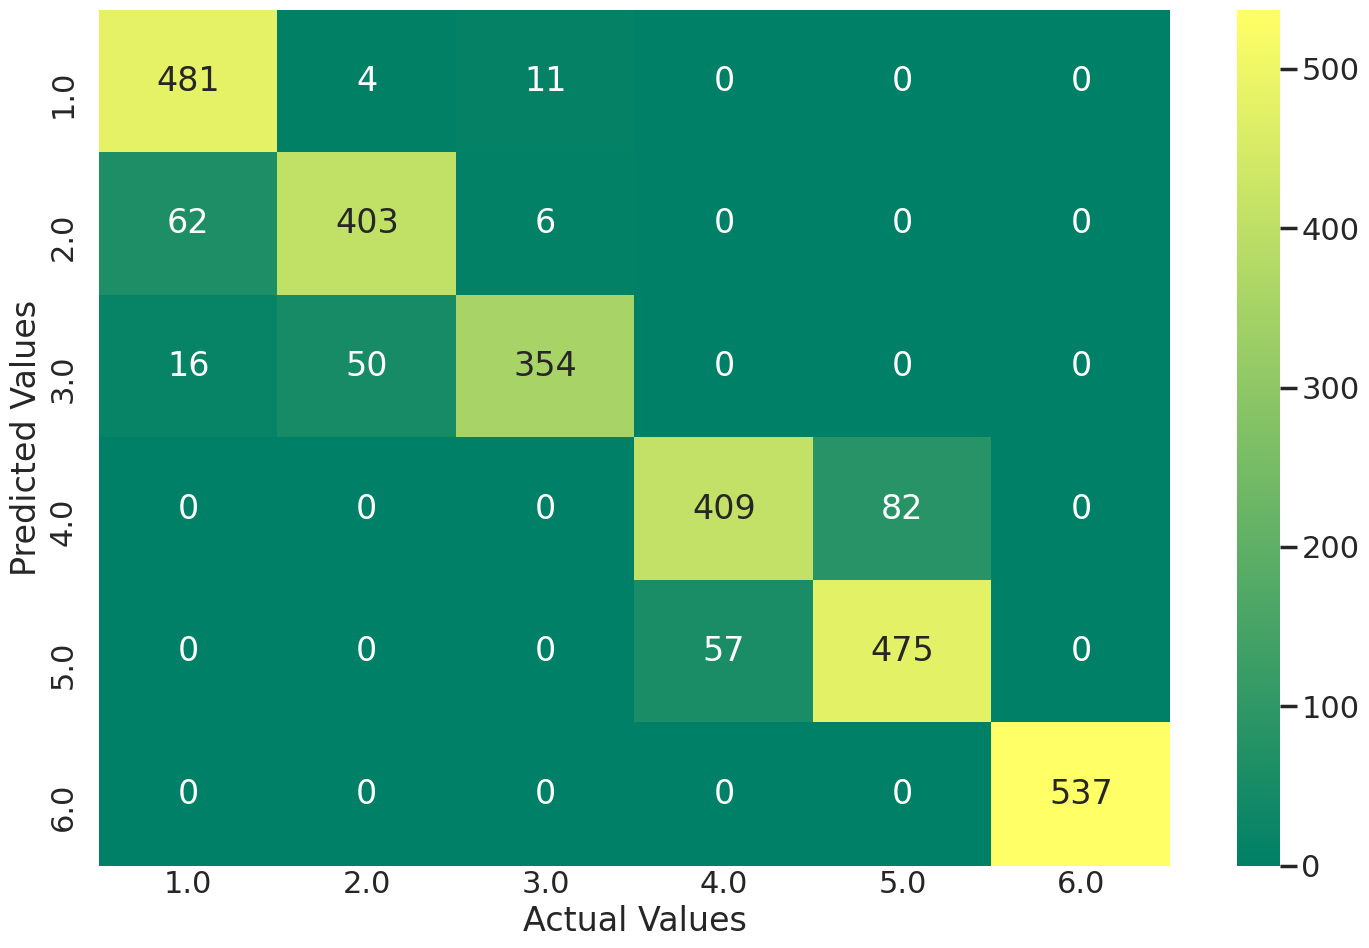
\includegraphics[width=\linewidth]{Img/ConfMat.png}
    \caption{Confusion matrix for the AdaBoost SAMME tested with the test data.}
    \label{fig:ConfMat}
\end{figure}

The AdaBoost SAMME accuracy and time to fit and test was also compared against the one versus one SVM, the decision tree, the random forest, and the KNN. The results can be viewed in Fig. \ref{fig:Barplot}.

\begin{figure}[tb]
    \centering
    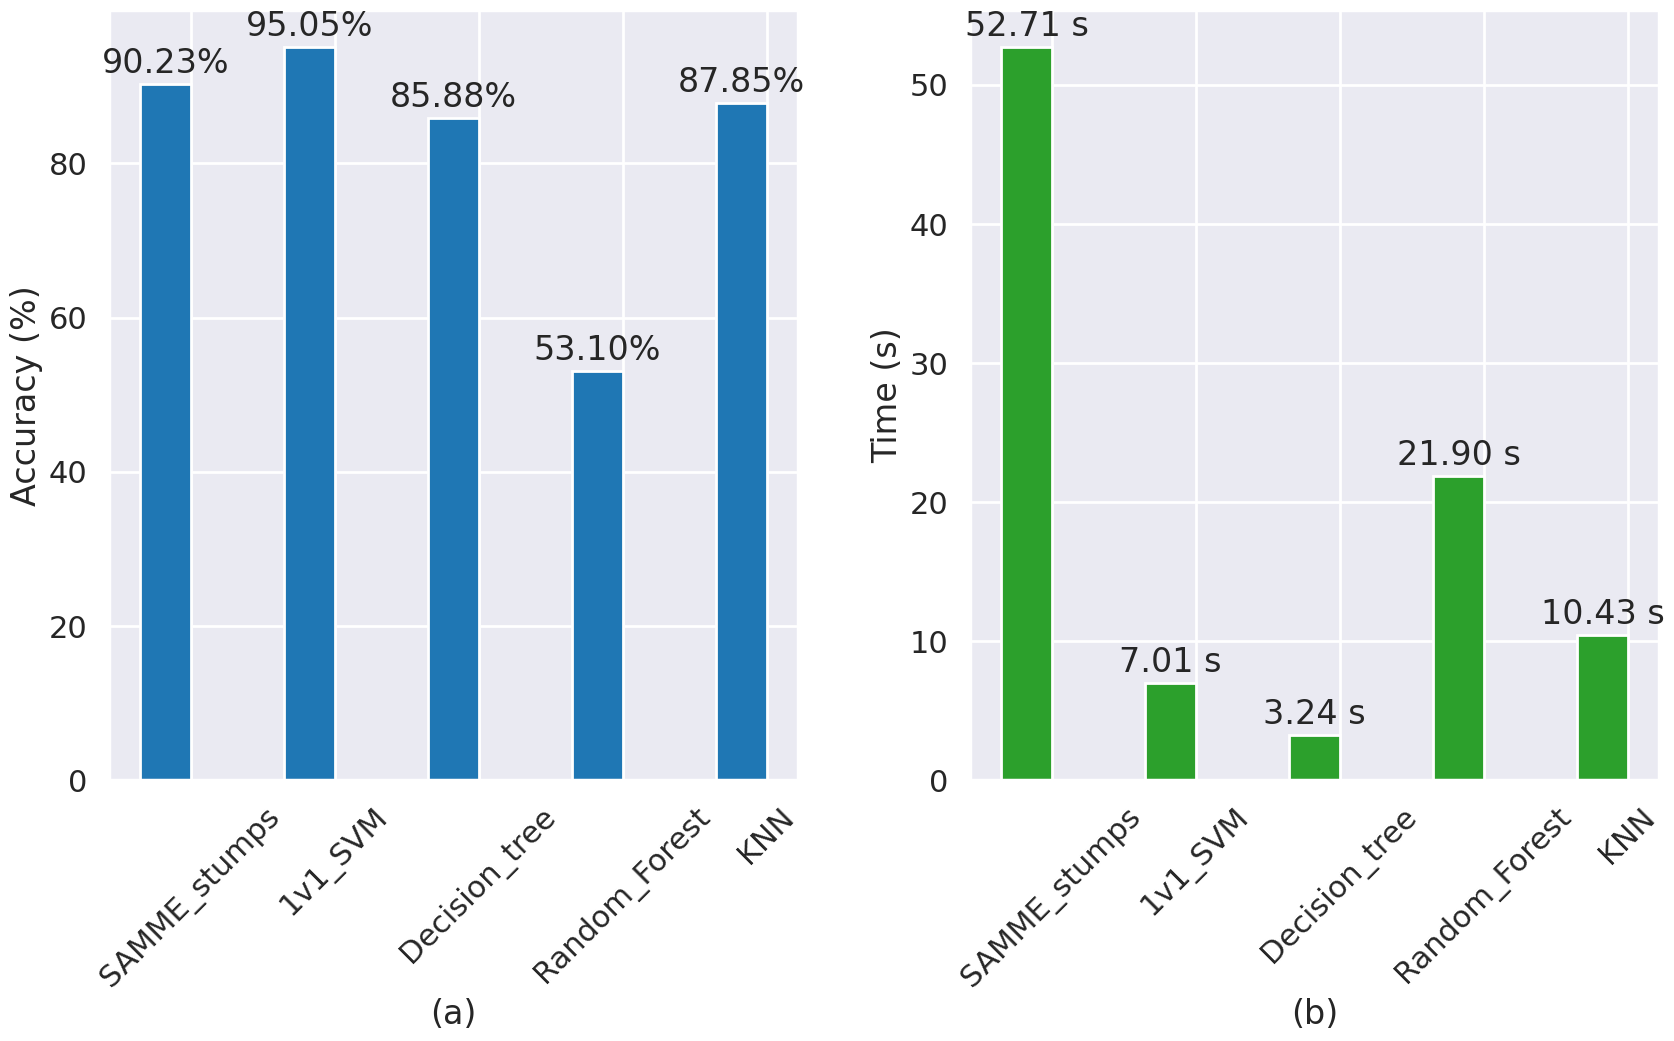
\includegraphics[width=\linewidth]{Img/Barplot.png}
    \caption{Accuracy (a) and time to fit and test (b) of each of the classifiers being compared against the AdaBoost SAMME.}
    \label{fig:Barplot}
\end{figure}


\subsection{Discussion}
Table \ref{tab:SAMME_comparison} shows that for those parameters, the best performing combination was using stumps with a classifier number of $2000$. Additionally, there seems to be a trend that indicates that larger values than $2000$ might also have increased accuracy, although this might be due to overfitting. 

Taking a look at the SVM, it also seems like the accuracy has not plateaued and could also be increased with a larger value for classifier number, however the 10-times 10-fold cross-validation time for $ClassifierNumber=200$ was calculated to be more than $8000$ seconds, and thus was discarded. Although SVM could in theory outperform the stumps approach, the time it takes to compute would be considerable and thus might not be useful for classification if there is a need for constant retraining of the model. Due to this, the combination of stump learner with $2000$ classifiers was selected.

The confusion matrix in Fig. \ref{fig:ConfMat} shows that although the performance of the classifier can be considered good, the system might have issues differentiating between class $5$ and class $4$, that according to the dataset description correspond to the activities of "sitting" and "standing", respectively. Although it seems that the classifier has difficulties differentiating between these two classes compared with the rest, the issue seems to be localized to just these classes and the average accuracy for them is approximately $86\%$, which can be argued is not a low score. The classifier seems to also misclassify some instances of class $1$, "walking", as class $2$, "walking upstairs", as well as misclassify instances of class $2$ as class $3$, "walking downstairs". This could be caused due to the amount of features present in the dataset and the classifier being only capable of creating decision trees with only one feature to separate the data. It is possible that this could be solved by increasing the depth of the tree, or using a technique that helps reduce the amounts of features in the dataset like Principal Component Analysis.

Additionally, Fig. \ref{fig:Barplot} seems to also indicate that the final accuracy for SAMME is $90.23\%$ on the test component of the dataset. It can be argued that this is a good accuracy, however it is still less than the results for the one versus one SVM at $95.05\%$. This might be due to the fact that the one vs one SVM has access to the complete dataset while training, while the SAMME AdaBoost is using approximately $700$ samples per iteration. Also, the time it took to compute the SAMME is much larger, a limitation present in the boosting algorithm as it cannot be parallelized due to its weight calculation for each classifier being dependent on the results from the previous iteration. 

Moreover, the SAMME algorithm also outperformed the decision tree classifier, again at the cost of a much higher computational time. This also indicates that it is possible that a larger depth could benefit greatly the performance of the SAMME algorithm, but the computational time could also increase dramatically.

Furthermore, it is also worth noting that SAMME did outperform the random forest classifier, as mentioned in the literature. However, the low accuracy of the random forest is also due to the use of stumps for training. Nonetheless, the random forest's benefit of being able to train all the trees simultaneously means that it is much faster than SAMME to fit and test, and thus could potentially be more useful in certain applications like embedded systems, depending on the depth of the trees used in both algorithms.

\subsection{Conclusion}
Although the best performing SAMME parameter combination was stumps and a classifier number of $2000$, there seems to be a likelihood of larger classifier numbers having a better accuracy as well. SAMME was able to outperform in accuracy the random forest, the decision tree and the KNN classifier, but at a higher computational time. One versus one SVM was the best performing classifier in both accuracy and time.

Additionally, further work in selecting different parameters for the weak learners should also be explored, e.g. changing the C value for the SVM and the depth of the trees on the decision tree, to evaluate their effect on the accuracy of the SAMME classifier. Furthermore, other weak learners might outperform the use of stumps or SVMs in the AdaBoost SAMME algorithm and should also be explored.

Finally, a more complex method like the AdaC2.M1 proposed in \cite{Sun_multiclass_inbalanced_AdaC2.M1} could be used instead of the SAMME algorithm for the multi-class classification.

% -----------------------b--------------------------------------------------
\bibliographystyle{IEEEbib}
\bibliography{strings,refs}

\end{document}
